\documentclass[12pt,]{article}
\usepackage{lmodern}
\usepackage{amssymb,amsmath,stmaryrd}
\usepackage{ifxetex,ifluatex}
\usepackage{fixltx2e} % provides \textsubscript
\ifnum 0\ifxetex 1\fi\ifluatex 1\fi=0 % if pdftex
  \usepackage[T1]{fontenc}
  \usepackage[utf8]{inputenc}
\else % if luatex or xelatex
  \ifxetex
    \usepackage{mathspec}
  \else
    \usepackage{fontspec}
  \fi
  \defaultfontfeatures{Ligatures=TeX,Scale=MatchLowercase}
\fi
% use upquote if available, for straight quotes in verbatim environments
\IfFileExists{upquote.sty}{\usepackage{upquote}}{}
% use microtype if available
\IfFileExists{microtype.sty}{%
\usepackage{microtype}
\UseMicrotypeSet[protrusion]{basicmath} % disable protrusion for tt fonts
}{}
\usepackage[margin=1in]{geometry}
\usepackage{hyperref}
\PassOptionsToPackage{usenames,dvipsnames}{color} % color is loaded by hyperref
\hypersetup{unicode=true,
            pdftitle={Extending ggplot2's grammar of graphics implementation for linked and dynamic graphics on the web},
            pdfauthor={Carson Sievert},
            pdfkeywords={Animation, Linked Views, Statistical graphics, Exploratory data
analysis, Web technologies},
            colorlinks=true,
            linkcolor=cyan,
            citecolor=black,
            urlcolor=Blue,
            breaklinks=true}
\urlstyle{same}  % don't use monospace font for urls
\usepackage{color}
\usepackage{fancyvrb}
\newcommand{\VerbBar}{|}
\newcommand{\VERB}{\Verb[commandchars=\\\{\}]}
\DefineVerbatimEnvironment{Highlighting}{Verbatim}{commandchars=\\\{\}}
% Add ',fontsize=\small' for more characters per line
\usepackage{framed}
\definecolor{shadecolor}{RGB}{248,248,248}
\newenvironment{Shaded}{\begin{snugshade}}{\end{snugshade}}
\newcommand{\KeywordTok}[1]{\textcolor[rgb]{0.13,0.29,0.53}{\textbf{#1}}}
\newcommand{\DataTypeTok}[1]{\textcolor[rgb]{0.13,0.29,0.53}{#1}}
\newcommand{\DecValTok}[1]{\textcolor[rgb]{0.00,0.00,0.81}{#1}}
\newcommand{\BaseNTok}[1]{\textcolor[rgb]{0.00,0.00,0.81}{#1}}
\newcommand{\FloatTok}[1]{\textcolor[rgb]{0.00,0.00,0.81}{#1}}
\newcommand{\ConstantTok}[1]{\textcolor[rgb]{0.00,0.00,0.00}{#1}}
\newcommand{\CharTok}[1]{\textcolor[rgb]{0.31,0.60,0.02}{#1}}
\newcommand{\SpecialCharTok}[1]{\textcolor[rgb]{0.00,0.00,0.00}{#1}}
\newcommand{\StringTok}[1]{\textcolor[rgb]{0.31,0.60,0.02}{#1}}
\newcommand{\VerbatimStringTok}[1]{\textcolor[rgb]{0.31,0.60,0.02}{#1}}
\newcommand{\SpecialStringTok}[1]{\textcolor[rgb]{0.31,0.60,0.02}{#1}}
\newcommand{\ImportTok}[1]{#1}
\newcommand{\CommentTok}[1]{\textcolor[rgb]{0.56,0.35,0.01}{\textit{#1}}}
\newcommand{\DocumentationTok}[1]{\textcolor[rgb]{0.56,0.35,0.01}{\textbf{\textit{#1}}}}
\newcommand{\AnnotationTok}[1]{\textcolor[rgb]{0.56,0.35,0.01}{\textbf{\textit{#1}}}}
\newcommand{\CommentVarTok}[1]{\textcolor[rgb]{0.56,0.35,0.01}{\textbf{\textit{#1}}}}
\newcommand{\OtherTok}[1]{\textcolor[rgb]{0.56,0.35,0.01}{#1}}
\newcommand{\FunctionTok}[1]{\textcolor[rgb]{0.00,0.00,0.00}{#1}}
\newcommand{\VariableTok}[1]{\textcolor[rgb]{0.00,0.00,0.00}{#1}}
\newcommand{\ControlFlowTok}[1]{\textcolor[rgb]{0.13,0.29,0.53}{\textbf{#1}}}
\newcommand{\OperatorTok}[1]{\textcolor[rgb]{0.81,0.36,0.00}{\textbf{#1}}}
\newcommand{\BuiltInTok}[1]{#1}
\newcommand{\ExtensionTok}[1]{#1}
\newcommand{\PreprocessorTok}[1]{\textcolor[rgb]{0.56,0.35,0.01}{\textit{#1}}}
\newcommand{\AttributeTok}[1]{\textcolor[rgb]{0.77,0.63,0.00}{#1}}
\newcommand{\RegionMarkerTok}[1]{#1}
\newcommand{\InformationTok}[1]{\textcolor[rgb]{0.56,0.35,0.01}{\textbf{\textit{#1}}}}
\newcommand{\WarningTok}[1]{\textcolor[rgb]{0.56,0.35,0.01}{\textbf{\textit{#1}}}}
\newcommand{\AlertTok}[1]{\textcolor[rgb]{0.94,0.16,0.16}{#1}}
\newcommand{\ErrorTok}[1]{\textcolor[rgb]{0.64,0.00,0.00}{\textbf{#1}}}
\newcommand{\NormalTok}[1]{#1}
\usepackage{longtable,booktabs}
\usepackage{graphicx,grffile}
\makeatletter
\def\maxwidth{\ifdim\Gin@nat@width>\linewidth\linewidth\else\Gin@nat@width\fi}
\def\maxheight{\ifdim\Gin@nat@height>\textheight\textheight\else\Gin@nat@height\fi}
\makeatother
% Scale images if necessary, so that they will not overflow the page
% margins by default, and it is still possible to overwrite the defaults
% using explicit options in \includegraphics[width, height, ...]{}
\setkeys{Gin}{width=\maxwidth,height=\maxheight,keepaspectratio}
\IfFileExists{parskip.sty}{%
\usepackage{parskip}
}{% else
\setlength{\parindent}{0pt}
\setlength{\parskip}{6pt plus 2pt minus 1pt}
}
\setlength{\emergencystretch}{3em}  % prevent overfull lines
\providecommand{\tightlist}{%
  \setlength{\itemsep}{0pt}\setlength{\parskip}{0pt}}
\setcounter{secnumdepth}{5}
% Redefines (sub)paragraphs to behave more like sections
\ifx\paragraph\undefined\else
\let\oldparagraph\paragraph
\renewcommand{\paragraph}[1]{\oldparagraph{#1}\mbox{}}
\fi
\ifx\subparagraph\undefined\else
\let\oldsubparagraph\subparagraph
\renewcommand{\subparagraph}[1]{\oldsubparagraph{#1}\mbox{}}
\fi

%%% Use protect on footnotes to avoid problems with footnotes in titles
\let\rmarkdownfootnote\footnote%
\def\footnote{\protect\rmarkdownfootnote}

% ------------------------------------------------------------------------------
% Start of JCGS specific titlepage
% ------------------------------------------------------------------------------


\usepackage{amsthm}
\newtheorem{theorem}{Theorem}[section]
\newtheorem{lemma}{Lemma}[section]
\theoremstyle{definition}
\newtheorem{definition}{Definition}[section]
\newtheorem{corollary}{Corollary}[section]
\newtheorem{proposition}{Proposition}[section]
\theoremstyle{definition}
\newtheorem{example}{Example}[section]
\theoremstyle{remark}
\newtheorem*{remark}{Remark}
\begin{document}

\def\spacingset#1{\renewcommand{\baselinestretch}%
{#1}\small\normalsize} \spacingset{1}

\title{\bf Extending ggplot2's grammar of graphics implementation for linked and
dynamic graphics on the web}
\author{
  Carson Sievert \\ 
  Department of Statistics, Iowa State University \\
  Toby Dylan Hocking \\ 
  Department of Human Genetics, McGill University \\
  Susan VanderPlas \\
  Department of Statistics, Iowa State University \\
  Jun Cai \\
  Department of Earth System Science, Tsinghua University\\
  Kevin Ferris \\
  Baseball Operations Department, Tampa Bay Rays
}
\maketitle

\bigskip
\begin{abstract}
% 200 or fewer words
The web is the most popular medium for sharing interactive data
visualizations thanks to the portability of the web browser and the
accessibility of the internet. Unfortunately, creating interactive web
graphics often requires a working knowledge of numerous web technologies
that are foreign to many people working with data. As a result, web
graphics are rarely used for exploratory data analysis where quick
iteration between different visualizations is of utmost importance. This
is the core strength of ggplot2, a popular data visualization package
for R, the world's leading open-source statistical programming language.
The conceptual framework behind ggplot2 is based on the grammar of
graphics, which lays a foundation for describing any static graphic as a
small set of independent components. Perhaps the most fundamental
component is the mapping from abstract data to the visual space,
sometimes referred to as the aesthetic mapping. We propose adding two
new aesthetics to the grammar, which together are sufficient for
elegantly describing both animations and certain classes of coordinated
linked views. We implement this extension in the open-source R package
animint, which converts ggplot2 objects to interactive web
visualizations via D3.
\end{abstract}

\noindent
{\it Keywords:}  Animation, Linked Views, Statistical graphics, Exploratory data
analysis, Web technologies
\vfill

\newpage
\spacingset{1.45} % DON'T change the spacing!

% ------------------------------------------------------------------------------
% End of JCGS specific titlepage
% ------------------------------------------------------------------------------

\section{Introduction}\label{intro}

The world's leading open source statistical programming language, R, has
a rich history of interfacing with computational tools for the use of
people doing data analysis and statistics research (R Core Team 2015).
Understanding R's core audience is important, as they typically want to
maximize their time working on data analysis problems, and minimize time
spent learning computational tools. R excels in this regard, as it is
designed specifically for interactive use, where users can quickly
explore their data using highly expressive interfaces. Another key
player in R's success story is its packaging infrastructure, which
provides tools for distributing entire research conpendium(s) (code,
data, documentation, auxiliary documents, etc) (Gentleman and Lang
2004).

One of the most widely used R packages is ggplot2, a data visualization
package inspired by the grammar of graphics (Wickham 2009, Wilkinson et
al. (2006)). In fact, Donoho (2015) writes: ``This effort may have more
impact on today's practice of data analysis than many highly-regarded
theoretical statistics papers''. In our experience, ggplot2 has made an
impact thanks to its foundation in the grammar of graphics, carefully
chosen defaults, and overall usability. This helps data analysts rapidly
iterate and discover informative visualizations -- an essential task in
exploratory data analysis (EDA). When dealing with high-dimensional
data, however, it is often useful to produce interactive and/or dynamic
graphics, which ggplot2 does not inherently support.

Interactive graphics toolkits in R have been used for decades to enhance
the EDA workflow, but these approaches are often not easy to reproduce
or distribute to a larger audience. It is true that most graphics
generated during EDA are ultimately not useful, but sometimes,
understanding gained during this phase is most easily shared via the
interactive graphics themselves. Thus, there is value in being able to
easily share, and embed interactive graphics inside a larger report.
Unfortunately, this is typically hard, if not impossible, using
traditional interactive graphics toolkits. As a result, there is a large
disconnect between the visualization tools that we use for exploration
versus presentation.

We aim to narrow this gap in visualization tools by extending ggplot2's
grammar of graphics implementation for interactive and dynamic web
graphics. Our extension allows one to create animated transitions and
perform dynamic queries via direct manipulation of linked views like
those described in Ahlberg, Williamson, and Shneiderman (1991) and Buja
et al. (1991). A conceptual model for our extension is provided in
Section \ref{extension} and Section \ref{animation}. In Section
\ref{worldbank}, we demonstrate our extension with an example. In
Section \ref{implementation}, we outline design decisions made in our
implementation in the R package animint. In Section \ref{performance},
we provide a sense of the scope of our system and its performance
limitations through a handful of examples. In Section \ref{compare}, we
conduct a comparison study by replicating examples with other leading
systems. Finally, in Section \ref{limitations}, we discuss future work
and limitations of our current system.

\section{Related Work}\label{related-work}

We aim to provide a system which empowers ggplot2 users to go beyond the
confines of static graphics with minimal friction imposed upon their
current workflow. We acknowledge that numerous systems which support
similar visualization techniques exist outside of the R ecosystem, but
we intentionally focus on R interfaces since the surrounding statistical
computing environment is crucial for enabling an efficient exploratory
data analysis workflow.

It is important to acknowledge that ggplot2 is built on top of the R
package grid, a low-level graphics system, which is now bundled with R
itself (R Core Team 2015). Neither grid, nor base R graphics, have
strong support for handling user interaction, which creates a need for
add-on packages. There are a number of approaches these packages take to
rendering, each with their own benefits and drawbacks. Traditionally,
they build on low-level R interfaces to graphical systems such as GTK+,
Qt, or Java GUI frameworks (Lawrence and Temple Lang 2010, Lawrence and
Sarkar (2016a), Lawrence and Sarkar (2016b), Urbanek (2016)). In
general, the resulting system can be very fast and flexible, but sharing
and reproducing output is usually a problem due to the heavy software
requirements. Although there may be sacrifices in performance, using the
modern web browser as a canvas is more portable, accessible, and
composable (graphics can be embedded within larger
frameworks/documents).

Base R does provide a Scalable Vector Graphics (SVG) device,
\texttt{svg()}, via the Cairo graphics API (Cairo 2016). The R package
SVGAnnotation provides functionality to post-process \texttt{svg()}
output in order to add interactive and dynamic features (Nolan and Lang
2012). This is a powerful approach, since in theory it can work with any
R graphic, but the package is self described as a proof-of-concept which
reverse engineers poorly structured \texttt{svg()} output. As a result,
anyone wishing to extend or alter the core functionality needs a deep
understanding of base graphics and SVG.

The lack of well-structured SVG for R graphics motivated the gridSVG
package which provides sensible structuring of SVG output for grid
graphics (Murrell and Potter 2015). This package also provides some
low-level tools for animating or adding interactive features, where grid
objects must be referenced by name. As a result, if one wanted to use
this interface to add interactivity to a ggplot2 plot, they must know
and understand the grid naming scheme ggplot2 uses internally and hope
it does not change down the road. An interface where interactivity can
be expressed by referencing the data to be visualized, rather than the
building blocks of the graphics system, would be preferable since the
former interface is decoupled from the implementation and does not
require knowledge of grid.

In terms of the animation API, the R package gganimate is very similar
to our system (Robinson 2016). It directly extends ggplot2 by adding a
new aesthetic, named \texttt{frame}, which splits the data into subsets
(one for each unique value of the frame variable), produces a static
plot for each subset, and uses the animation package to combine the
images into a key frame animation (Xie 2013). This is quite similar, but
not as flexible as our system's support for animation, which we fully
describe in Section \ref{animation}. Either system has the ability to
control the amount of time that a given frame is displayed, but our
system can also animate the transition between frames via the
\texttt{d3.transition()} API (Bostock, Oglevetsky, and Heer 2011).
Smooth transitions help us track positions between frames, which is
useful in many scenarios, such as the touring example discussed in
Section \ref{tour}.

Tours are a useful visualization technique for exploring
high-dimensional data which requires interactive and dynamic graphics.
The open source software ggobi is currently the most fully-featured tool
for touring data and has support for interactive techniques such as
linking, zooming, panning, and identifying (Cook and Swayne 2007). The R
package rggobi (Wickham et al. 2008) provides an R interface to ggobi's
graphical interface, but unfortunately, the software requirements for
installation and use of this toolchain are heavy and stringent.
Furthermore, sharing the interactive versions of these graphics are not
possible. The R package cranvas aims to be the successor to ggobi, with
support for similar interactive techniques, but with a more flexible
interface for describing plots inspired by the grammar of graphics (Xie
et al. 2013). Cranvas also has heavy and stringent software requirements
which limits the portability and accessibility of the software.

Another R package for interactive graphics which draws design
inspiration from the grammar of graphics is ggvis (Chang and Wickham
2015). It does not directly extend ggplot2, but instead provides a brand
new purely functional interface which is designed with interactive
graphics in mind. It currently relies on Vega to render the SVG graphics
from JSON (Trifacta 2014), and the R package shiny to enable many of its
interactive capabilities (RStudio 2013). The interface gives tremendous
power to R users, as it allows one to write R functions to handle user
events. This power does come with a cost, though, as sharing and hosting
ggvis graphics typically requires special web server software, even when
the interaction logic could be handled entirely client-side. As we
outline in Section \ref{implementation}, our system does not require a
web server, but can also be used inside shiny web applications, when
desired.

\section{Extending the layered grammar of
graphics}\label{extending-the-layered-grammar-of-graphics}

In this section, we propose an extension to the layered grammar of
graphics (Wickham 2010), which enables declarative expression of
animations and dynamic queries via direct manipulation. In the ggplot2
system, there are five essential components that define a layer of
graphical makings: data, mappings (i.e., aesthetics), geometry,
statistic, and position. These simple components are easily understood
in isolation and can be combined in many ways to express a wide array of
graphics. For a simple example, here is one way to create a scatterplot
in ggplot2 of variables named \texttt{\textless{}X\textgreater{}} and
\texttt{\textless{}Y\textgreater{}} in
\texttt{\textless{}DATA\textgreater{}}:

\begin{Shaded}
\begin{Highlighting}[]
\KeywordTok{ggplot}\NormalTok{() }\OperatorTok{+}\StringTok{ }\KeywordTok{layer}\NormalTok{(}
  \DataTypeTok{data =} \OperatorTok{<}\NormalTok{DATA}\OperatorTok{>}\NormalTok{, }
  \DataTypeTok{mapping =} \KeywordTok{aes}\NormalTok{(}\DataTypeTok{x =} \OperatorTok{<}\NormalTok{X}\OperatorTok{>}\NormalTok{, }\DataTypeTok{y =} \OperatorTok{<}\NormalTok{Y}\OperatorTok{>}\NormalTok{), }
  \DataTypeTok{geom =} \StringTok{"point"}\NormalTok{, }
  \DataTypeTok{stat =} \StringTok{"identity"}\NormalTok{,}
  \DataTypeTok{position =} \StringTok{"identity"}
\NormalTok{)}
\end{Highlighting}
\end{Shaded}

For every geometry, ggplot2 provides a convenient wrapper around
\texttt{layer()} which provides sensible defaults for the statistic and
position (in this case, both are ``identity''):

\begin{Shaded}
\begin{Highlighting}[]
\KeywordTok{ggplot}\NormalTok{() }\OperatorTok{+}\StringTok{ }\KeywordTok{geom_point}\NormalTok{(}
  \DataTypeTok{data =} \OperatorTok{<}\NormalTok{DATA}\OperatorTok{>}\NormalTok{, }
  \KeywordTok{aes}\NormalTok{(}\DataTypeTok{x =} \OperatorTok{<}\NormalTok{X}\OperatorTok{>}\NormalTok{, }\DataTypeTok{y =} \OperatorTok{<}\NormalTok{Y}\OperatorTok{>}\NormalTok{)}
\NormalTok{)}
\end{Highlighting}
\end{Shaded}

A single ggplot2 plot can be comprised of multiple layers, and different
layers can correspond to different data. Since each graphical mark
within a ggplot2 layer corresponds to one (or more) observations in
\texttt{\textless{}DATA\textgreater{}}, aesthetic mappings provide a
mechanism for mapping graphical selections to the original data (and
vice-versa) which is essential to any interactive graphics system
(Andreas Buja and McDonald 1988, Wickham et al. (2010)). Thus, given a
way to combine multiple ggplot2 plots into a single view, this design
can be extended to support a notion of multiple linked views, as those
discussed in Ahlberg, Williamson, and Shneiderman (1991) and Buja et al.
(1991).

\subsection{Direct Manipulation of Dynamic Queries}\label{extension}

Cook and Swayne (2007) use SQL queries to formalize the direct
manipulation methods discussed in Ahlberg, Williamson, and Shneiderman
(1991) and Buja et al. (1991). As it turns out, we can embed this
framework inside the layered grammar of graphics with two classes of new
aesthetics: one class to define a selection source and one to define a
target. This is most easily seen using our animint implementation, which
has a \texttt{clickSelects} aesthetic for defining the selection source
(via mouse click) and a \texttt{showSelected} aesthetic for defining the
target. Here we use animint to create a linked view between a bar chart
and a scatter plot, where the user can click on bars to control the
points shown in the scatterplot, as shown in the video in Figure
\ref{fig:tips}. As a result, we can quickly see how the relationship
among tip amount and total bill amount depends on whether the customer
is smoker.

\begin{Shaded}
\begin{Highlighting}[]
\KeywordTok{library}\NormalTok{(animint)}
\NormalTok{p1 <-}\StringTok{ }\KeywordTok{ggplot}\NormalTok{() }\OperatorTok{+}\StringTok{ }\KeywordTok{geom_bar}\NormalTok{(}
  \DataTypeTok{data =}\NormalTok{ reshape2}\OperatorTok{::}\NormalTok{tips, }
  \KeywordTok{aes}\NormalTok{(}\DataTypeTok{x =}\NormalTok{ smoker, }\DataTypeTok{clickSelects =}\NormalTok{ smoker)}
\NormalTok{)}
\NormalTok{p2 <-}\StringTok{ }\KeywordTok{ggplot}\NormalTok{() }\OperatorTok{+}\StringTok{ }\KeywordTok{geom_point}\NormalTok{(}
  \DataTypeTok{data =}\NormalTok{ reshape2}\OperatorTok{::}\NormalTok{tips, }
  \KeywordTok{aes}\NormalTok{(}\DataTypeTok{x =}\NormalTok{ total_bill, }\DataTypeTok{y =}\NormalTok{ tip, }
      \DataTypeTok{showSelected =}\NormalTok{ smoker)}
\NormalTok{)}
\KeywordTok{animint2dir}\NormalTok{(}\KeywordTok{list}\NormalTok{(}\DataTypeTok{p1 =}\NormalTok{ p1, }\DataTypeTok{p2 =}\NormalTok{ p2))}
\end{Highlighting}
\end{Shaded}

\begin{figure}
\centering
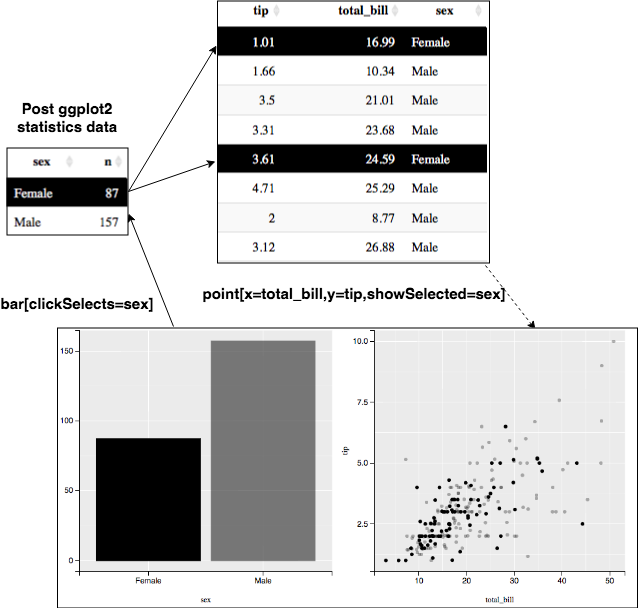
\includegraphics{images/tips}
\caption{\label{fig:tips}Linked dynamic querying via direct manipulation
using animint. A video demonstration can be viewed online at
\url{https://vimeo.com/160496419}}
\end{figure}

In essense, the R code above allows us to use direct manipulation to
dynamically perform SQL queries of the form:

\begin{Shaded}
\begin{Highlighting}[]
\KeywordTok{SELECT}\NormalTok{ total_bill, tip }\KeywordTok{FROM}\NormalTok{ tips}
  \KeywordTok{WHERE}\NormalTok{ smoker }\KeywordTok{IN}\NormalTok{ clickSelects}
\end{Highlighting}
\end{Shaded}

In this example, \texttt{clickSelects} is either ``Yes'' or ``No'', but
as we show in later examples, \texttt{clickSelects} can also be an array
of values. Although \texttt{clickSelects} is tied to a mouseclick event,
this same framework supports other selection events, such as hover or
click+drag. Statistically speaking, this is useful for visualizing and
navigating through joint distributions conditional upon discrete values.
In this sense, our extension is closely related to trellis displays and
linked scatterplot brushing (Becker, Cleveland, and Shyu 2010, Becker
and Cleveland (1987)). The major differences are that our conditioning
is layer-specific (not plot-specific), is not tied to a particular
geometry, and can be controlled through direct manipulation or animation
controls.

\subsection{Adding animation}\label{animation}

In some sense, the \texttt{showSelected} aesthetic splits the layer into
subsets -- one for every unique value of the \texttt{showSelected}
variable. The \texttt{clickSelects} aesthetic provides a mechanism to
alter the visibility of those subset(s) via direct manipulation, but our
system also provides a mechanism for automatically looping through
selections to produce animation(s). We achieve this by reserving the
name \texttt{time} to specify which variable to select as well as the
amount of time to wait before changing the selection (in milliseconds).
We also reserve the name \texttt{duration} to specify the amount of time
used to smoothly transition between frames (with linear easing). The
code below is used to generate Figure \ref{fig:animation} which
demonstrates a simple animation with smooth transitions between 10
frames of a single point. Note that the resulting web page has controls
for interactively altering the \texttt{time} and \texttt{duration}
parameters.

\begin{Shaded}
\begin{Highlighting}[]
\NormalTok{d <-}\StringTok{ }\KeywordTok{data.frame}\NormalTok{(}\DataTypeTok{v =} \DecValTok{1}\OperatorTok{:}\DecValTok{10}\NormalTok{)}
\NormalTok{plotList <-}\StringTok{ }\KeywordTok{list}\NormalTok{(}
  \DataTypeTok{plot =} \KeywordTok{ggplot}\NormalTok{() }\OperatorTok{+}\StringTok{ }\KeywordTok{geom_point}\NormalTok{(}
    \DataTypeTok{data =}\NormalTok{ d, }\KeywordTok{aes}\NormalTok{(}\DataTypeTok{x =}\NormalTok{ v, }\DataTypeTok{y =}\NormalTok{ v, }\DataTypeTok{showSelected =}\NormalTok{ v)}
\NormalTok{  ),}
  \DataTypeTok{time =} \KeywordTok{list}\NormalTok{(}\DataTypeTok{variable =} \StringTok{"v"}\NormalTok{, }\DataTypeTok{ms =} \DecValTok{1000}\NormalTok{),}
  \DataTypeTok{duration =} \KeywordTok{list}\NormalTok{(}\DataTypeTok{v =} \DecValTok{1000}\NormalTok{)}
\NormalTok{)}
\KeywordTok{animint2dir}\NormalTok{(plotList)}
\end{Highlighting}
\end{Shaded}

\begin{figure}
\centering
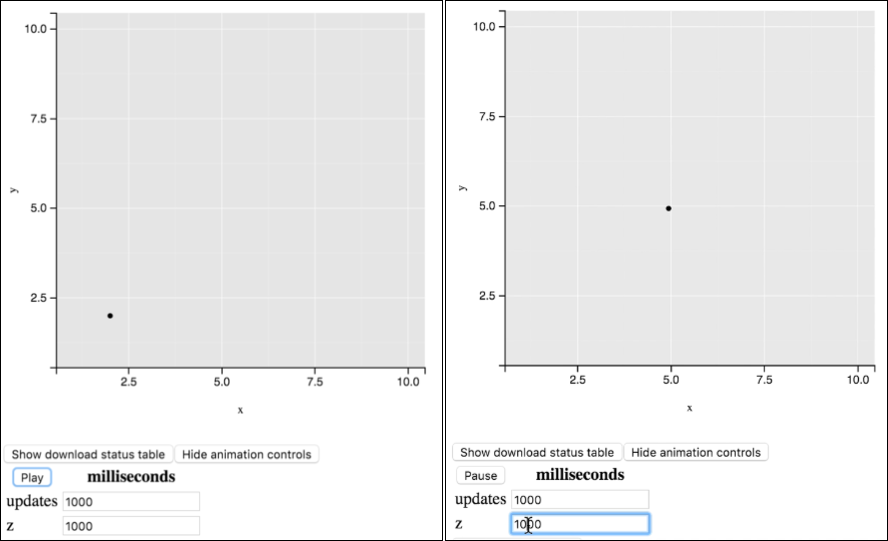
\includegraphics{images/animation}
\caption{\label{fig:animation}A simple animation with smooth transitions and
interactively altering transition durations. A video demonstration can
be viewed online at \url{https://vimeo.com/160505146}}
\end{figure}

\subsection{World Bank Example}\label{worldbank}

Figure \ref{fig:worldbank} shows an interactive animation of the World
Bank data set created with our animint implementation (World Bank 2012).
The visualization helps us explore the change in the relationship
between life expectancy and fertility over time for 205 countries. By
default, the year 1979 and the countries United States and Vietnam are
selected, but readers are encouraged to watch the video of the animation
and/or interact the visualization using a web
browser.\footnote{\url{http://bl.ocks.org/tdhock/raw/8ce47eebb3039263878f/}}
In the interactive version, the selected value of the year variable is
automatically incremented every few seconds, using animation to
visualize yearly changes in the relationship between life expectancy and
fertility rate.

\begin{figure}
\centering
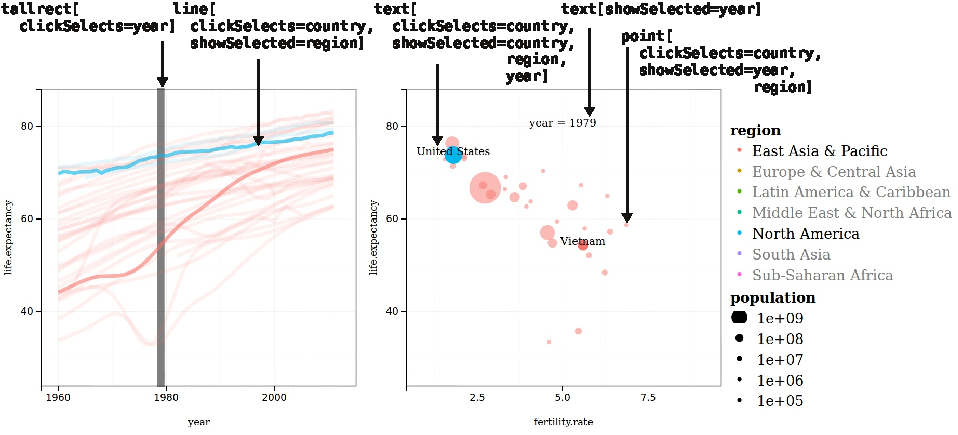
\includegraphics{images/figure-1.pdf}
\caption{\label{fig:worldbank}An interactive animation of World Bank
demographic data of several countries, designed using
\texttt{clickSelects} and \texttt{showSelected} keywords (top). Left: a
multiple time series from 1960 to 2010 of life expectancy, with bold
lines showing the selected countries and a vertical grey tallrect
showing the selected year. Right: a scatterplot of life expectancy
versus fertility rate of all countries. The legend and text elements
show the current selection: year=1979, country=\{United States,
Vietnam\}, and region=\{East Asia \& Pacific, North America\}}
\end{figure}

When viewing the interactive version of Figure \ref{fig:worldbank},
suppose we wish to select Thailand. Direct manipulation is not very
useful in this case since it is not easy to identify and select Thailand
based on graphical marks on a plot. For this reason, animint also
provides dropdown menu(s) for each selection variable to aid the
selection process. Figure \ref{fig:widgets} shows what the user sees
after typing ``th'' in the search box. Note that these dropdowns support
selection of multiple values and coordinate sensibly with selections
made via direct manipulation.

\begin{figure}
\centering
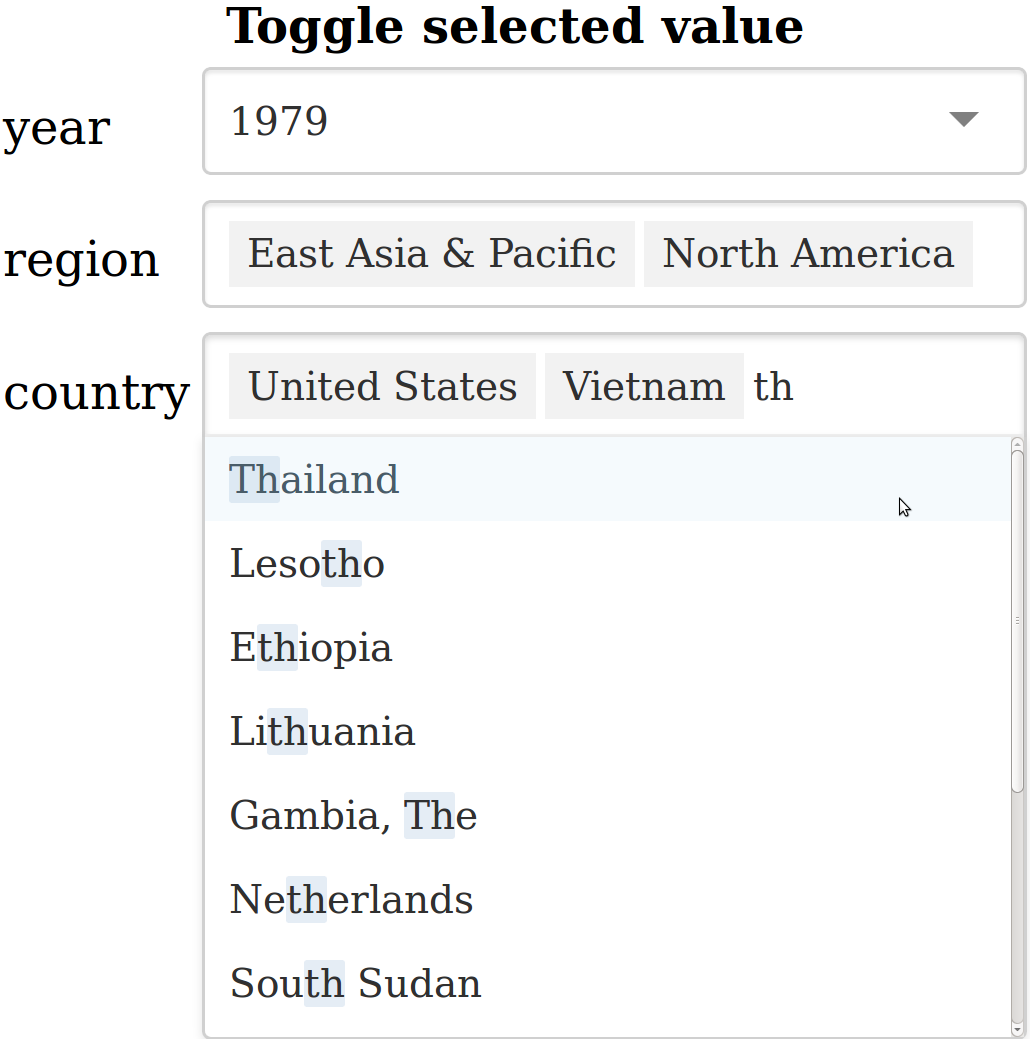
\includegraphics{images/Screenshot-toggle-selected-value}
\caption{\label{fig:widgets}Animint provides a menu to update each selection
variable. In this example, after typing `th' the country menu shows the
subset of matching countries.}
\end{figure}

We anticipate that some ggplot2 users will be able to reverse engineer
the animint code which creates Figure \ref{fig:worldbank}, simply by
looking at it. In fact, this is a big reason why ggplot2 is so widely
used: it helps minimize the amount of time required to translate a
figure that exists in your head into computer code. Note that, in the
left hand plot of Figure \ref{fig:worldbank}, we have a time series of
the life expectancy where each line is a country (i.e., we
\texttt{group} by country) and lines are colored by region. By clicking
on a line, we also want the country label to appear in the right hand
plot, so we also need to set \texttt{clickSelects=country}. Lastly, by
setting \texttt{showSelected=region}, we can hide/show lines by clicking
on the color legend entries.

\begin{Shaded}
\begin{Highlighting}[]
\NormalTok{timeSeries <-}\StringTok{ }\KeywordTok{ggplot}\NormalTok{() }\OperatorTok{+}\StringTok{ }\KeywordTok{geom_line}\NormalTok{(}
  \DataTypeTok{data =}\NormalTok{ WorldBank,}
  \KeywordTok{aes}\NormalTok{(}\DataTypeTok{x =}\NormalTok{ year, }\DataTypeTok{y =}\NormalTok{ life.expectancy,}
      \DataTypeTok{group =}\NormalTok{ country, }\DataTypeTok{color =}\NormalTok{ region,}
      \DataTypeTok{clickSelects =}\NormalTok{ country, }
      \DataTypeTok{showSelected =}\NormalTok{ region)}
\NormalTok{)}
\end{Highlighting}
\end{Shaded}

We want to provide a visual cue for the selected year in the time
series, so in the code below we add some tall rectangles to the time
series plot. These tall rectangles will also serve as a way to directly
modify the selected year. The tallrect geometry is a special case of a
rectangle that automatically spans the entire vertical range, so we just
have to specify the horizontal range via xmin and xmax. Also, since the
layered grammar of graphics allows for different data in each layer, we
supply a data frame with just the unique years in the entire data for
this layer.

\begin{Shaded}
\begin{Highlighting}[]
\NormalTok{years <-}\StringTok{ }\KeywordTok{data.frame}\NormalTok{(}\DataTypeTok{year =} \KeywordTok{unique}\NormalTok{(WorldBank}\OperatorTok{$}\NormalTok{year))}
\NormalTok{timeSeries <-}\StringTok{ }\NormalTok{timeSeries }\OperatorTok{+}\StringTok{ }\KeywordTok{geom_tallrect}\NormalTok{(}
  \DataTypeTok{data =}\NormalTok{ years,}
  \KeywordTok{aes}\NormalTok{(}\DataTypeTok{xmin =}\NormalTok{ year }\OperatorTok{-}\StringTok{ }\FloatTok{0.5}\NormalTok{, }\DataTypeTok{xmax =}\NormalTok{ year }\OperatorTok{+}\StringTok{ }\FloatTok{0.5}\NormalTok{,}
      \DataTypeTok{clickSelects =}\NormalTok{ year)}
\NormalTok{)}
\end{Highlighting}
\end{Shaded}

As for the right hand plot in Figure \ref{fig:worldbank}, there are
three layers: a point layer for countries, a text layer for countries,
and a text layer to display the selected year. By clicking on a point,
we want to display the country text label and highlight the
corresponding time series on the left hand plot, so we set
\texttt{clickSelects=country} in this layer. Furthermore, we only want
to show the points for the selected year and region, so we also need
\texttt{showSelected=year} and \texttt{showSelected2=region}.

\begin{Shaded}
\begin{Highlighting}[]
\NormalTok{scatterPlot <-}\StringTok{ }\KeywordTok{ggplot}\NormalTok{() }\OperatorTok{+}\StringTok{ }\KeywordTok{geom_point}\NormalTok{(}
  \DataTypeTok{data =}\NormalTok{ WorldBank,}
  \KeywordTok{aes}\NormalTok{(}\DataTypeTok{x =}\NormalTok{ fertility.rate, }\DataTypeTok{y =}\NormalTok{ life.expectancy,}
      \DataTypeTok{color =}\NormalTok{ region, }\DataTypeTok{size =}\NormalTok{ population,}
      \DataTypeTok{clickSelects =}\NormalTok{ country,}
      \DataTypeTok{showSelected =}\NormalTok{ year,}
      \DataTypeTok{showSelected2 =}\NormalTok{ region)}
\NormalTok{)}
\end{Highlighting}
\end{Shaded}

The text layer for annotating selected countries is essentially the same
as the point layer, except we map the country name to the \texttt{label}
aesthetic.

\begin{Shaded}
\begin{Highlighting}[]
\NormalTok{scatterPlot <-}\StringTok{ }\NormalTok{scatterPlot }\OperatorTok{+}\StringTok{ }\KeywordTok{geom_text}\NormalTok{(}
  \DataTypeTok{data =}\NormalTok{ WorldBank,}
  \KeywordTok{aes}\NormalTok{(}\DataTypeTok{x =}\NormalTok{ fertility.rate, }\DataTypeTok{y =}\NormalTok{ life.expectancy,}
      \DataTypeTok{label =}\NormalTok{ country,}
      \DataTypeTok{showSelected =}\NormalTok{ country,}
      \DataTypeTok{showSelected2 =}\NormalTok{ year,}
      \DataTypeTok{showSelected3 =}\NormalTok{ region)}
\NormalTok{)}
\end{Highlighting}
\end{Shaded}

Lastly, to help identify the selected year when viewing the scatterplot,
we add another layer of text at a fixed location.

\begin{Shaded}
\begin{Highlighting}[]
\NormalTok{scatterPlot <-}\StringTok{ }\NormalTok{scatterPlot }\OperatorTok{+}\StringTok{ }\KeywordTok{geom_text}\NormalTok{(}
  \DataTypeTok{data =}\NormalTok{ years, }\DataTypeTok{x =} \DecValTok{5}\NormalTok{, }\DataTypeTok{y =} \DecValTok{80}\NormalTok{,}
  \KeywordTok{aes}\NormalTok{(}\DataTypeTok{label =} \KeywordTok{paste}\NormalTok{(}\StringTok{"year = "}\NormalTok{, year),}
      \DataTypeTok{showSelected =}\NormalTok{ year)}
\NormalTok{)}
\end{Highlighting}
\end{Shaded}

Now that we have defined the plots in Figure \ref{fig:worldbank}, we can
set the \texttt{time} and \texttt{duration} options (introduced in
Section \ref{animation}) to control the animation parameters. Our
animint implementation also respects a \texttt{selector.types} option
which controls whether or not selections for a given variable can
accumulate and a \texttt{first} option for controlling which values are
selected by default.
\footnote{We maintain a complete list of (animint specific) options here -- \url{https://github.com/tdhock/animint/wiki/Advanced-features-present-animint-but-not-in-ggplot2}}
By default, supplying the list of plots and additional options to
\texttt{animint2dir()} will write all the files necessary to render the
visualization to a temporary directory and prompt a web browser to open
an HTML file.

\begin{Shaded}
\begin{Highlighting}[]
\NormalTok{viz <-}\StringTok{ }\KeywordTok{list}\NormalTok{(}
  \DataTypeTok{timeSeries =}\NormalTok{ timeSeries,}
  \DataTypeTok{scatterPlot =}\NormalTok{ scatterPlot,}
  \DataTypeTok{time =} \KeywordTok{list}\NormalTok{(}\DataTypeTok{variable =} \StringTok{"year"}\NormalTok{, }\DataTypeTok{ms =} \DecValTok{3000}\NormalTok{),}
  \DataTypeTok{duration =} \KeywordTok{list}\NormalTok{(}\DataTypeTok{year =} \DecValTok{1000}\NormalTok{),}
  \DataTypeTok{selector.types =} \KeywordTok{list}\NormalTok{(}
    \DataTypeTok{year =} \StringTok{"single"}\NormalTok{,}
    \DataTypeTok{country =} \StringTok{"multiple"}\NormalTok{,}
    \DataTypeTok{region =} \StringTok{"multiple"}
\NormalTok{  ),}
  \DataTypeTok{first =} \KeywordTok{list}\NormalTok{(}
    \DataTypeTok{country =} \KeywordTok{c}\NormalTok{(}\StringTok{"United States"}\NormalTok{, }\StringTok{"Vietnam"}\NormalTok{)}
\NormalTok{  )}
\NormalTok{)}
\KeywordTok{animint2dir}\NormalTok{(viz)}
\end{Highlighting}
\end{Shaded}

\subsection{Implementation details}\label{implementation}

As shown in Figure \ref{fig:design}, the animint system is implemented
in 2 parts: the compiler and the renderer. The compiler is implemented
in about 2000 lines of R code that converts a list of ggplots and
options to a JSON plot meta-data file and a tab-separated values (TSV)
file database.

\begin{figure}
\centering
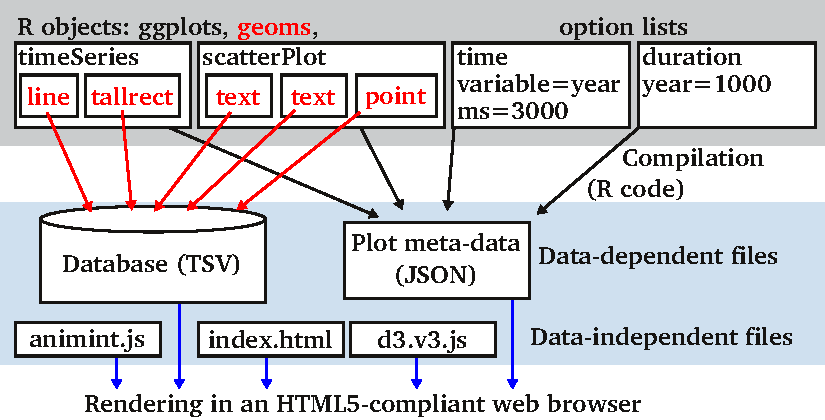
\includegraphics{images/figure-design.pdf}
\caption{\label{fig:design}A schematic explanation of compilation and
rendering in the World Bank visualization. Top: the interactive
animation is a list of 4 R objects: 2 ggplots and 2 option lists.
Center: animint R code compiles data in ggplot geoms to a database of
TSV files (\textcolor{red}{$\rightarrowtriangle$}). It also compiles
plot meta-data including ggplot aesthetics, animation time options, and
transition duration options to a JSON meta-data file
(\(\rightarrowtriangle\)). Bottom: those data-dependent compiled files
are combined with data-independent JavaScript and HTML files which
render the interactive animation in a web browser
(\textcolor{blue}{$\rightarrowtriangle$}).}
\end{figure}

\begin{figure}
\centering
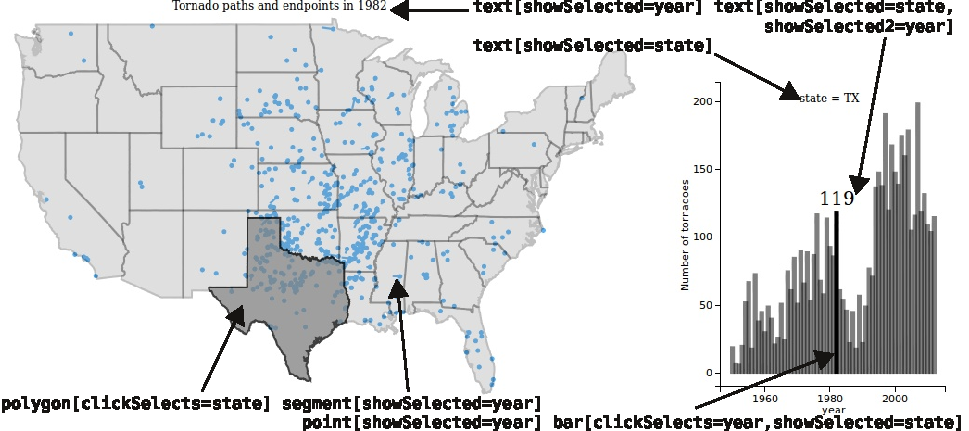
\includegraphics{images/figure-tornado.pdf}
\caption{\label{fig:tornado}Interactive animation of tornadoes recorded from
1950 to 2012 in the United States. Left: map of the lower 48 United
States with tornado paths in 1982. The text shows the selected year, and
clicking the map changes the selected state, currently Texas. Right:
time series of tornado counts in Texas. Clicking a bar changes the
selected year, and the text shows selected state and the number of
tornadoes recorded there in that year (119 tornadoes in Texas in 1982).}
\end{figure}

\begin{figure}
\centering
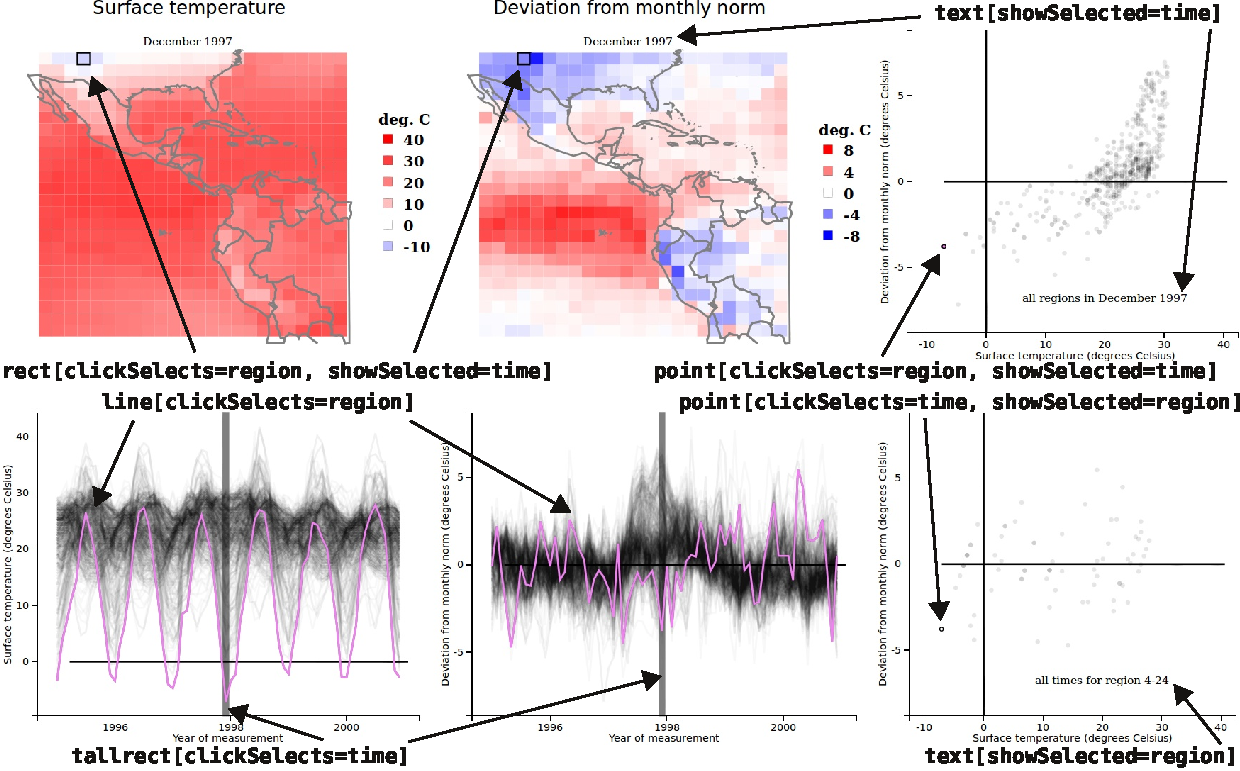
\includegraphics{images/figure-climate.pdf}
\caption{\label{fig:climate}Visualization containing 6 linked, interactive,
animated plots of Central American climate data. Top: for the selected
time (December 1997), maps displaying the spatial distribution of two
temperature variables, and a scatterplot of these two variables. The
selected region is displayed with a black outline, and can be changed by
clicking a rect on the map or a point on the scatterplot. Bottom: time
series of the two temperature variables with the selected region shown
in violet, and a scatterplot of all times for that region. The selected
time can be changed by clicking a background tallrect on a time series
or a point on the scatterplot. The selected region can be changed by
clicking a line on a time series.}
\end{figure}

The compiler scans the aesthetics in the ggplots to determine how many
selection variables are present, and which geoms to update after a
selection variable is updated. It uses ggplot2 to automatically
calculate the axes scales, legends, labels, backgrounds, and borders. It
outputs this information to the JSON plot meta-data file.

The compiler also uses ggplot2 to convert data variables (e.g.~life
expectancy and region) to visual properties (e.g.~y position and color).
The data for each layer/geom are saved in several TSV files, one for
each combination showSelected values. Thus for large data sets, the web
browser only needs to download the subset of data required to render the
current selection (Heer 2013).

When repeated data would be saved in each of the TSV files, an extra
common TSV file is created so that the repeated data only need to be
stored and downloaded once. In that case, the other TSV files do not
store the common data, but are merged with the common data after
downloading. This method for constructing the TSV file database was
developed to minimize the disk usage of animint, particularly for
ggplots of spatial maps as in Figure \ref{fig:tornado}.

Finally, the rendering engine (\texttt{index.html}, \texttt{d3.v3.js},
and \texttt{animint.js} files) is copied to the plot directory. The
\texttt{animint.js} renderer is implemented in about 2200 lines of
JavaScript/D3 code that renders the TSV and JSON data files as SVG in a
web browser. Importantly, animation is achieved by using the JavaScript
\texttt{setInterval()} function, which updates the \texttt{time}
selection variable every few seconds. Since the compiled plot is just a
directory of files, the interactive plots can be hosted on any web
server. The interactive plots can be viewed by opening the
\texttt{index.html} page in any modern web browser.

\section{Exploring performance \& scope with
examples}\label{performance}

This section attempts to demonstrate a range of visualizations that are
supported by animint with more examples. Figure \ref{fig:tornado} shows
an interactive animation of tornadoes observed in the United States
between 1950 and 2012. At any moment in time, the user can
simultaneously view the spatial distribution of tornadoes in the
selected year over all states, and see the trend over all years for the
selected state. Clicking a state on the map updates the time series bars
to show the tornado counts from that state. Clicking a bar on the time
series updates the selected year. Figure \ref{fig:climate} shows an
interactive animation of climate time series data observed in Central
America. Two maps display the spatial distribution of two temperature
variables, which are shown over time in corresponding the time series
plots below. Scatterplots also show the relationships between the two
temperature variables for the selected time and region. Clicking any of
the plots updates all 6 of them. The \texttt{clickSelects} and
\texttt{showSelected} aesthetics make it easy to design this set of 6
linked plots in only 87 lines of code.

Summary statistics describing complexity and performance for examples in
this paper, as well as other animint examples, are displayed in Table
\ref{tab:examples}. The climate data visualization has noticeably slow
animations, since it displays about 88,980 geometric elements at once
(\url{http://bit.ly/QcUrhn}). We observed this slowdown across all
browsers, which suggested that there is an inherent bottleneck when
rendering large interactive plots in web browsers using JavaScript and
SVG. Another animint with a similar amount of total rows is based on the
evolution data (\url{http://bit.ly/O0VTS4}), but since it shows less
data onscreen (about 2,703 elements), it exhibits faster responses to
interactivity and animation.

Animint is still useful for creating interactive but non-animated plots
when there is not a time variable in the data. In fact, 7 of the 11
examples in Table \ref{tab:examples} are not animated. For example,
linked plots are useful to illustrate complex concepts such as a change
point detection model in the breakpoints data
(\url{http://bit.ly/1gGYFIV}). The user can explore different model
parameters and data sets since these are encoded as animint interaction
variables.

\begin{table*}[htp] % This table is too wide to fill in the page.
  \centering
  % latex table generated in R 3.1.1 by xtable 1.7-3 package
% Thu Oct  9 14:20:02 2014
\begin{tabular}{rrrrrrrrrrr}
  \hline
 & LOC & seconds & MB & rows & onscreen & variables & interactive & plots & animated? & Fig \\ 
  \hline
worldPop & 17 & 0.2 & 0.1 & 924 & 624 &  4 &  2 &  2 & yes &  \\ 
  WorldBank & 20 & 2.3 & 2.1 & 34132 & 11611 &  6 &  2 &  2 & yes &  \ref{fig:worldbank} \\ 
  evolution & 25 & 21.6 & 12.0 & 240600 & 2703 &  5 &  2 &  2 & yes &  \\ 
  change & 36 & 2.8 & 2.5 & 36238 & 25607 & 12 &  2 &  3 & no &  \\ 
  tornado & 39 & 1.7 & 6.1 & 103691 & 16642 & 11 &  2 &  2 & no &  \ref{fig:tornado} \\ 
  prior & 54 & 0.7 & 0.2 & 1960 & 142 & 12 &  3 &  4 & no &  \\ 
  compare & 66 & 10.7 & 7.9 & 133958 & 2140 & 20 &  2 &  5 & no &  \\ 
  breakpoints & 68 & 0.5 & 0.3 & 4242 & 667 & 13 &  2 &  3 & no &  \\ 
  climate & 84 & 12.8 & 19.7 & 253856 & 88980 & 15 &  2 &  6 & yes &  \ref{fig:climate} \\ 
  scaffolds & 110 & 56.3 & 78.5 & 618740 & 9051 & 30 &  3 &  3 & no &  \\ 
  ChIPseq & 229 & 29.9 & 78.3 & 1292464 & 1156 & 44 &  4 &  5 & no & \\ 
   \hline
\end{tabular}

  \vskip 0.2cm
  \caption{Characteristics of 11 interactive visualizations designed with
    animint. The interactive version of these visualizations can be accessed 
    via \url{http://members.cbio.ensmp.fr/~thocking/animint/}.
    From left to right, we show the data set name, the
    lines of R code (LOC) including data processing but not including comments
    (80 characters max per line),
    the amount of time it takes to compile the visualization (seconds),
    the total size of the uncompressed TSV files in megabytes (MB),
    the total number of data points (rows),
    the median number of data points shown at once (onscreen),
    the number of data columns visualized (variables),
    the number of \texttt{clickSelects}/\texttt{showSelected} 
    variables (interactive),
    the number of linked panels (plots),
    if the plot is animated,
    and the corresponding Figure number in this paper (Fig).
  }
\label{tab:examples}
\end{table*}

\section{Comparison study}\label{compare}

In this section we compare our animint implementation with other similar
leading systems by creating a given visualization in each system and
discussing the pros and cons of the different approaches.

\subsection{The Grand Tour}\label{tour}

The Grand Tour is a well-known method for viewing high dimensional data
which requires interactive and dynamic graphics (Asimov 1985). Figure
\ref{fig:tour} shows a grand tour of 300 observations sampled from a
correlated tri-variate normal distribution. The left hand view shows the
marginal density of each point while the right hand view ``tours"
through 2D projections of the 3D data. There are many ways to choose
projections in a tour, and many ways to interpolate between projections,
most of which can be programmed fairly easily using R and relevant
add-on packages. In this case, we used the R package tourr, which uses
the geodesic random walk (i.e., random 2D projection with geodesic
interpolation) in its grand tour algorithm (Wickham et al. 2011).

\begin{figure}
\centering
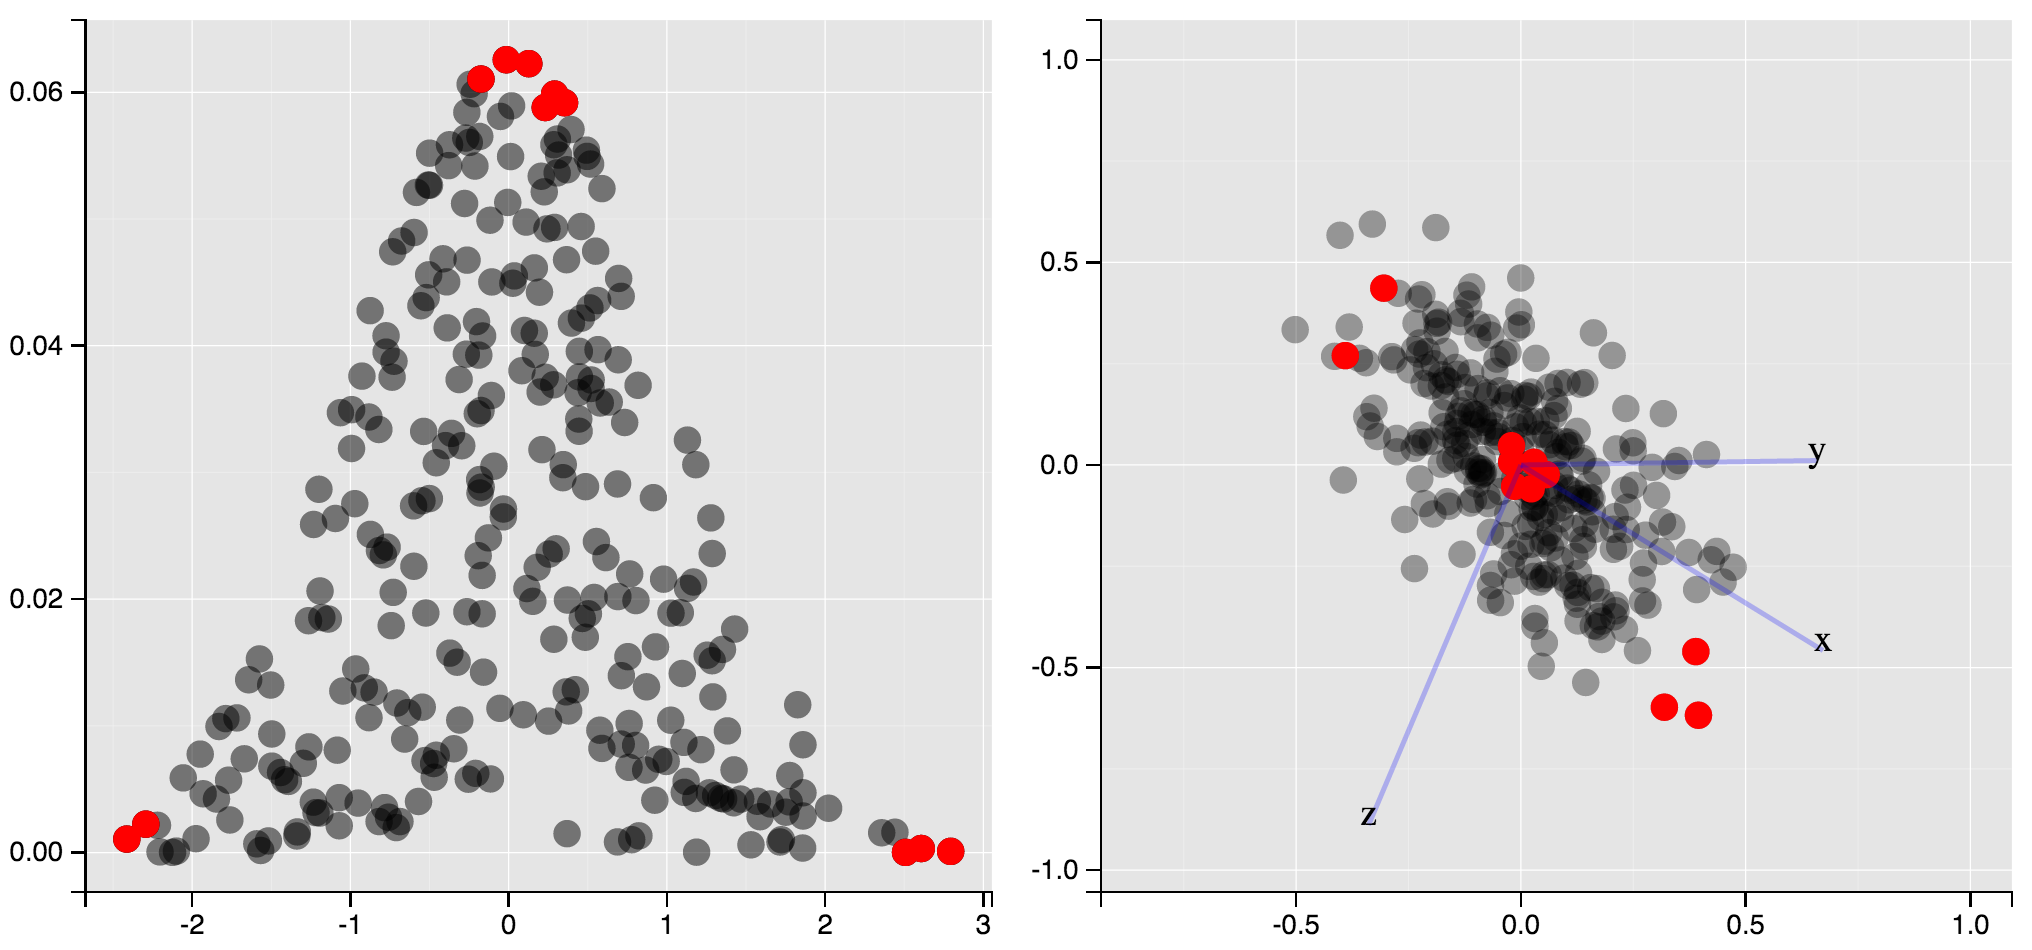
\includegraphics{images/tour}
\caption{\label{fig:tour}Linked selection in a grand tour with animint. A
video demonstration can be viewed online at
\url{https://vimeo.com/160720834}}
\end{figure}

When touring data, it is generally useful to link low-dimensional
displays with the tour itself. The video in Figure \ref{fig:tour} was
generated with our current animint implementation, and points are
selected via mouse click which reveals that points with high marginal
density are located in the ellipsoid center while points with a low
marginal density appear near the ellipsoid border. In this case, it
would be convenient to also have brush selection, as we demonstrate in
Figure \ref{fig:tourbrush} which imdplements the same touring example
using the R packages ggvis and shiny. The brush in Figure
\ref{fig:tourbrush} is implemented with shiny's support for brushing
static images, which currently does not support multiple brushes, making
it difficult to select non-contiguous regions.

\begin{figure}
\centering
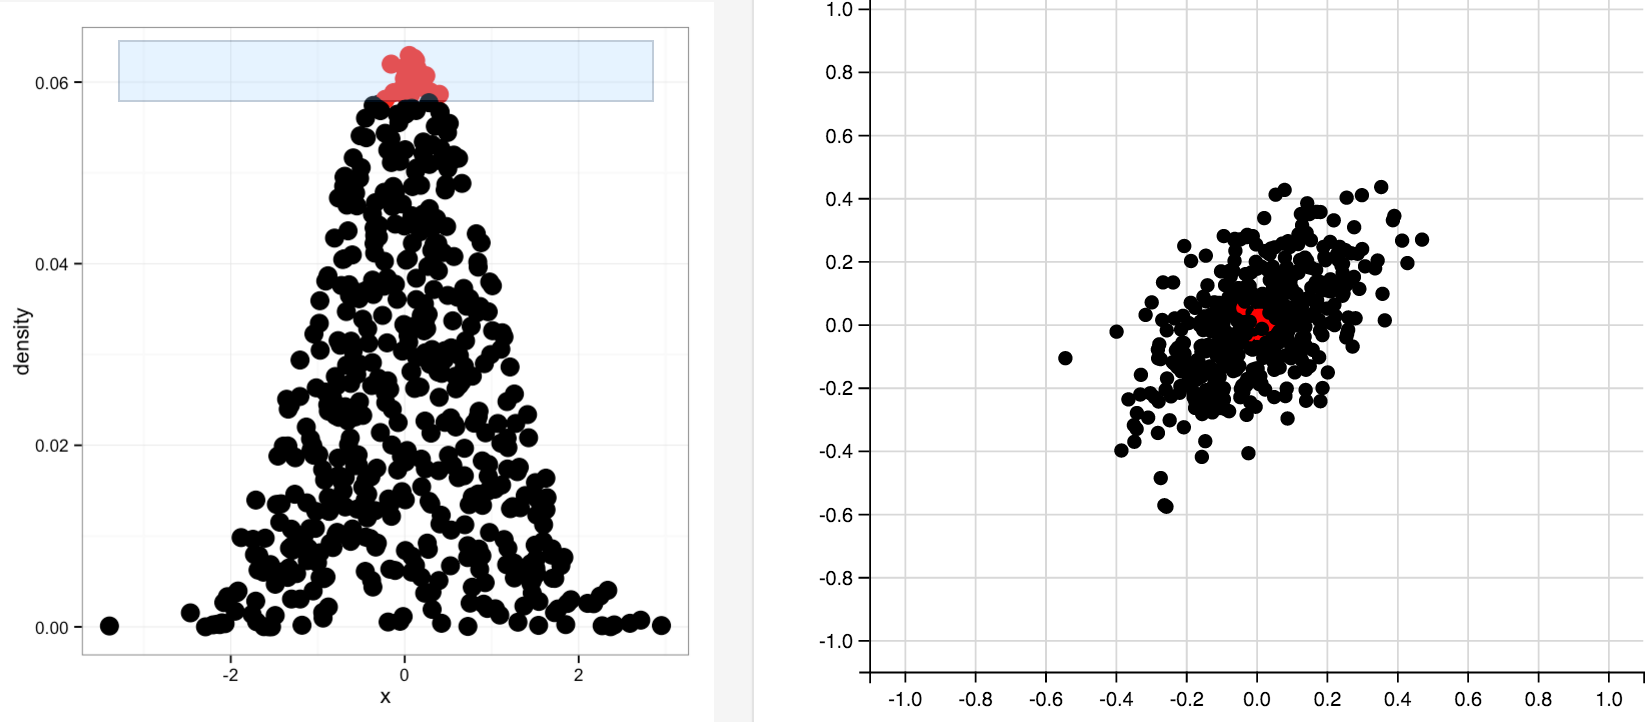
\includegraphics{images/tourbrush}
\caption{\label{fig:tourbrush}Linked selection in a grand tour with ggvis
and shiny. A video demonstration can be viewed online at
\url{https://vimeo.com/160825528}}
\end{figure}

This example helps point out a few other important differences in using
animint versus ggvis+shiny to implement `multiple linked and dynamic
views' as described in Ahlberg, Williamson, and Shneiderman (1991) and
Buja et al. (1991). Maintaining state of the linked brush in Figure
\ref{fig:tourbrush} requires both knowledge and clever use of some
sophicated programming techniques such as closures and reactivity. It
also requires knowledge of the shiny web application framework and a new
approach to the grammar of graphics. On the other hand, maintaining
state in Figure \ref{fig:tour} requires a few different
\texttt{clickSelects}/\texttt{showSelected} mappings. As a result, we
believe animint provides a more elegant user interface for this
application.

The touring example also helps point out important consequences of the
design and implementation of these two different systems. As mentioned
in Section \ref{implementation}, our current animint implementation
requires every subset of data to be precomputed before render time. For
visualizations such as tours, where it is more efficient to perform
statistical computations on-the-fly, this can be a harsh restriction,
but this is a restriction of our current implementation (not a
restriction of the framework itself). As a result, when touring a large
high-dimensional space, where many projections are needed, ggvis+shiny
may be desirable since the projections are computed on the server and
sent to the browser in real-time. This works fine when the application
is running and viewed on the same host machine, but viewing such an
application hosted on a remote machine can produce staggered animations
since client-server requests must be performed, processed, and rendered
roughly 30 times a second. Also, generally speaking, the animint system
results a more pleasant experience when it comes to hosting and sharing
applications since it doesn't require a Web Server with R and special
software already installed.

\subsection{World Bank Example}\label{world-bank-example}

We also recreated Figure \ref{fig:worldbank} using ggvis+shiny (see
\url{http://bit.ly/1SsJKlN}) and Tableau (see
\url{http://bit.ly/worldBank-tableau}). Even as experienced ggvis+shiny
users, we found it quite difficult to replicate this example, and were
not able completely replicate it due to a lack of a mechanism for
coordinating indirect and direct manipulations. Overall the
visualization is pretty similar, but lacks a few important features. In
particular, there is no way to control the selected year using both the
slider (indirect) and clicking on the ggvis plot (direct). It also lacks
the ability to click on a country time series and label the
corresponding point on the scatterplot. This might be possible, but we
could not find a way to update a plot based on a click event on a
different plot. Even with this lack of functionality, the ggvis+shiny is
significantly more complicated and requires more code (about 100 lines
of code compared to 30).

It was also impossible to completely replicate Figure
\ref{fig:worldbank} using Tableau essentially because the example
requires a \emph{layered} approach to the grammar of graphics. In
particular, since graphical marks and interaction source/target(s) must
derive from the same table in Tableau, it was impossible to control the
clickable multiple time series and the clickable tallrects in different
ways based on the two different selection variables. In other words, in
Tableau, selections are managed on the plot level, but in animint,
selections are specific to each graphical layer.

\section{User feedback and
observations}\label{user-feedback-and-observations}

By working with researchers in several fields of research, we have
created a wide variety of interactive visualizations using animint.
Typically, the researchers have a complex data set that they wish to
visualize, but they do not have the expertise or time to create an
interactive data visualization. The animint system made it easy to
collaborate with the various domain experts, who were able to provide us
with annotated sketches of the desired plots, which we then translated
to animint R code. In this section we share comments and constructive
criticisms that we have obtained from our users.

\subsection{User perspective}\label{user-perspective}

For the \texttt{prior} data visualization (\url{http://bit.ly/1peIT7t}),
the animint user is a machine learning researcher who developed an
algorithm and applied it to 4 benchmark data sets. He wanted to explore
how his algorithm performed, in comparison to a baseline learning
algorithm. He appreciated the intuition about his algorithm's
performance that he learned from the interactive plots: ``Interactive
plotting allows us to explore all relationships of our high-dimensional
dataset and gives us an intuitive understanding of the performance of
our proposed algorithm. An intuitive understanding of the results is
important since it shows under which conditions our proposed method
works well and provides avenues for further research.''

Another user from a machine learning background found the interactive
plots useful for presenting his work: ``the `regularization path' is a
difficult concept to demonstrate in my research. The animint
(\url{http://bit.ly/1gVb8To}) helped greatly by rendering an interactive
plot of regularization path, likelihood, and graph at the same time and
illustrating their connections. It also reveals an interesting
phenomenon that maximizing the testing likelihood actually gives many
false positives.''

In another application, the animint user was a genomics researcher:
``viewing and exploring my complex intestinal microbiome dataset in
animint allowed me to grasp the patterns and relationships between
samples at an almost intuitive level. The interactive aspect of it was
very helpful for browsing through the dataset.''

Finally, users also appreciated the simple web interface, and the detail
that is possible to show in interactive plots, but impossible to show in
publications: ``\ldots{} the web interface is simple and easy to use. It
also enables us to publish more detailed interactive results on our
website to accompany the results presented in publications.''

\subsection{Developer perspective}\label{developer-perspective}

R users, and in particular ggplot2 users, have found that animint is
easy to learn and use. One statistics Ph.D.~student writes, ``animint is
a fantastic framework for creating interactive graphics for someone
familiar with R and ggplot2's grammar of graphics implementation. The
API is very intuitive and allows one to quickly bring their static
graphics to life in a way that facilitates exploratory data analysis.''

\section{Limitations and future work}\label{limitations}

A number of limitations derive from the fact that some plot features are
computed once during the compilation step and remain static on a
rendered plot. For example, users are unable to change variable mappings
after compilation. Also, when different data subsets have very different
ranges of values, it may be preferable to recompute scales when
\texttt{clickSelects} selection(s) change. A future implementation of
animint would benefit from changes to the compiler and renderer that
allow scales to be updated after each click. Some of these limitations
can be resolved by adding interactive widgets to ``recompile" components
hard-coded in the plot meta information. In fact, animint makes it easy
to embed visualizations inside of shiny web applications, and we have an
example of interactively redefining variable mappings
(\url{http://bit.ly/animint-shiny}).

Our compiler also currently takes advantage of ggplot2 internals to
compute statistics and positional adjustments before rendering. As a
result, statistics/positions will not dynamically recompute based on
selections. In other words, using
\texttt{clickSelects}/\texttt{showSelected} with non-identity
statistic(s)/position(s) may not generate a sensible result. It would be
possible, but a significant amount of work, to transfer these
computations from the compiler to the renderer.

Another set of limitations derive from our current restriction that all
subsets (corresponding to each possible selection) must be precomputed
before render time. As elucidated in Section \ref{tour}, if there is a
large space of possible selections, it is impractical to precompute
every subset before viewing. Therefore, it would be useful if the
renderer could dynamically compute subsets when new selections are made.

Our implementation is also limited to two specific types of direct
manipulation: selecting graphical elements via mouse click
(\texttt{clickSelects}), and showing/hiding related elements
(\texttt{showSelected}). However, the framework described in Section
\ref{extension} is not restricted to a particular event type, so
\texttt{hoverSelects} and \texttt{brushSelects} aesthetics could be
added, for instance. There are other types of interaction that should be
added, that wouldn't require additional extensions to the grammar of
graphics, such as: zooming, panning, and plot resizing.

\section{Conclusion}\label{conclusion}

Our R package animint extends ggplot2's layered grammar of graphics
implementation for a declarative approach to producing interactive and
dynamic web graphics. By adding two aesthetics to specify selection
source(s) and target(s), ggplot2 users can quickly and easily create
animations with smooth transitions and perform dynamic queries via
direct manipulation of linked views. As a result, animint is a useful
tool not only for exploratory data analysis, but also for the
presentation and distribution of interactive statistical graphics.

\section*{Acknowledgements}

The authors wish to thank animint users MC Du Plessis, Song Liu,
Nikoleta Juretic, and Eric Audemard who have contributed constructive
criticisms and helped its development.

\section*{References}

\hypertarget{refs}{}
\hypertarget{ref-Ahlberg:1991}{}
Ahlberg, Christopher, Christopher Williamson, and Ben Shneiderman. 1991.
``Dynamic Queries for Information Exploration: An Implementation and
Evaluation.'' In \emph{Proceedings of the Sigchi Conference on Human
Factors in Computing Systems}, 21:619--26.

\hypertarget{ref-viewing-pipeline}{}
Andreas Buja, Catherine Hurley, Daniel Asimov, and John A. McDonald.
1988. ``Elements of a Viewing Pipeline for Data Analysis.'' In
\emph{Dynamic Graphics for Statistics}, edited by William S. Cleveland
and Marylyn E. McGill. Belmont, California: Wadsworth, Inc.

\hypertarget{ref-grand-tour}{}
Asimov, Daniel. 1985. ``The Grand Tour: A Tool for Viewing
Multidimensional Data.'' \emph{SIAM J. Sci. Stat. Comput.} 6 (1).
Philadelphia, PA, USA: Society for Industrial; Applied Mathematics:
128--43. doi:\href{https://doi.org/10.1137/0906011}{10.1137/0906011}.

\hypertarget{ref-brushing-scatterplots}{}
Becker, RA, and WS Cleveland. 1987. ``Brushing Scatterplots.''
\emph{Technometrics} 29 (2): 127--42.

\hypertarget{ref-trellis}{}
Becker, Richard A., William S. Cleveland, and Ming-Jen Shyu. 2010. ``The
Visual Design and Control of Trellis Displays.'' \emph{Journal of
Computational and Graphical Statistics} 19 (1). Taylor \& Francis:
3--28.

\hypertarget{ref-d3}{}
Bostock, Michael, Vadim Oglevetsky, and Jeffrey Heer. 2011. ``D3
Data-Driven Documents.'' \emph{IEEE Transactions on Visualization and
Computer Graphics} 17 (12): 2301--9.

\hypertarget{ref-Buja:1991vh}{}
Buja, Andreas, John Alan McDonald, John Michalak, and Werner Stuetzle.
1991. ``Interactive data visualization using focusing and linking.''
\emph{IEEE Proceedings of Visualization}, February, 1--8.

\hypertarget{ref-cairo}{}
Cairo. 2016. ``Cairo: A Vector Graphics Library.''
\url{http://cairographics.org/}.

\hypertarget{ref-ggvis}{}
Chang, Winston, and Hadley Wickham. 2015. \emph{Ggvis: Interactive
Grammar of Graphics}. \url{https://CRAN.R-project.org/package=ggvis}.

\hypertarget{ref-ggobi:2007}{}
Cook, Dianne, and Deborah F. Swayne. 2007. \emph{Interactive and Dynamic
Graphics for Data Analysis : With R and Ggobi}. Use R ! New York:
Springer. \url{http://www.ggobi.org/book/}.

\hypertarget{ref-Donoho:2015tu}{}
Donoho, David. 2015. ``50 years of Data Science.''
\url{https://dl.dropboxusercontent.com/u/23421017/50YearsDataScience.pdf}.

\hypertarget{ref-Gentleman:Lang}{}
Gentleman, Robert, and Duncan Temple Lang. 2004. ``Statistical Analyses
and Reproducible Research.'' \emph{Bioconductor Project Working Papers},
November, 1--38.

\hypertarget{ref-2013-immens}{}
Heer, Zhicheng Liu AND Biye Jiang AND Jeffrey. 2013. ``ImMens: Real-Time
Visual Querying of Big Data.'' \emph{Computer Graphics Forum (Proc.
EuroVis)} 32 (3). \url{http://vis.stanford.edu/papers/immens}.

\hypertarget{ref-qtbase}{}
Lawrence, Michael, and Deepayan Sarkar. 2016a. \emph{Interface Between R
and Qt}. \url{https://github.com/ggobi/qtbase}.

\hypertarget{ref-qtpaint}{}
---------. 2016b. \emph{Qt-Based Painting Infrastructure}.
\url{https://github.com/ggobi/qtpaint}.

\hypertarget{ref-RGtk2}{}
Lawrence, Michael, and Duncan Temple Lang. 2010. ``RGtk2: A Graphical
User Interface Toolkit for R.'' \emph{Journal of Statistical Software}
37 (8): 1--52. \url{http://www.jstatsoft.org/v37/i08/}.

\hypertarget{ref-gridSVG}{}
Murrell, Paul, and Simon Potter. 2015. \emph{GridSVG: Export 'Grid'
Graphics as Svg}. \url{https://CRAN.R-project.org/package=gridSVG}.

\hypertarget{ref-SVGAnnotation}{}
Nolan, Deborah, and Duncan Temple Lang. 2012. ``Interactive and Animated
Scalable Vector Graphics and R Data Displays.'' \emph{Journal of
Statistical Software} 46 (1): 1--88.
\url{http://www.jstatsoft.org/v46/i01/}.

\hypertarget{ref-RCore}{}
R Core Team. 2015. \emph{R: A Language and Environment for Statistical
Computing}. Vienna, Austria: R Foundation for Statistical Computing.
\url{http://www.R-project.org/}.

\hypertarget{ref-gganimate}{}
Robinson, David. 2016. \emph{Gganimate: Create Easy Animations with
Ggplot2}. \url{http://github.com/dgrtwo/gganimate}.

\hypertarget{ref-shiny}{}
RStudio. 2013. ``Shiny: Easy Web Applications in R.''
\url{http://www.rstudio.com/shiny/}.

\hypertarget{ref-vega}{}
Trifacta. 2014. ``Vega: A Declarative Visualization Grammar.''
\url{http://trifacta.github.io/vega/}.

\hypertarget{ref-rJava}{}
Urbanek, Simon. 2016. \emph{RJava: Low-Level R to Java Interface}.
\url{https://CRAN.R-project.org/package=rJava}.

\hypertarget{ref-ggplot2-book}{}
Wickham, Hadley. 2009. \emph{Ggplot2: Elegant Graphics for Data
Analysis}. Springer New York. \url{http://had.co.nz/ggplot2/book}.

\hypertarget{ref-ggplot2-paper}{}
---------. 2010. ``A Layered Grammar of Graphics.'' \emph{Journal of
Computational and Graphical Statistics} 19 (1). Taylor \& Francis:
3--28.

\hypertarget{ref-tourr}{}
Wickham, Hadley, Dianne Cook, Heike Hofmann, and Andreas Buja. 2011.
``tourr: An R Package for Exploring Multivariate Data with
Projections,'' April, 1--18.

\hypertarget{ref-plumbing}{}
Wickham, Hadley, Michael Lawrence, Dianne Cook, Andreas Buja, Heike
Hofmann, and Deborah F Swayne. 2010. ``The Plumbing of Interactive
Graphics.'' \emph{Computational Statistics}, April, 1--7.

\hypertarget{ref-rggobi}{}
Wickham, Hadley, Michael Lawrence, Duncan Temple Lang, and Deborah F
Swayne. 2008. ``An Introduction to Rggobi.'' \emph{R-News} 8 (2): 3--7.
\url{http://CRAN.R-project.org/doc/Rnews/Rnews_2008-2.pdf}.

\hypertarget{ref-wilkinson}{}
Wilkinson, Leland, D Wills, D Rope, A Norton, and R Dubbs. 2006.
\emph{The Grammar of Graphics}. Springer.

\hypertarget{ref-WorldBank}{}
World Bank. 2012. ``World Development Indicators.''
\url{http://data.worldbank.org/data-catalog/world-development-indicators}.

\hypertarget{ref-animation}{}
Xie, Yihui. 2013. ``animation: An R Package for Creating Animations and
Demonstrating Statistical Methods.'' \emph{Journal of Statistical
Software} 53 (1): 1--27. \url{http://www.jstatsoft.org/v53/i01/}.

\hypertarget{ref-cranvas}{}
Xie, Yihui, Heike Hofmann, Di Cook, Xiaoyue Cheng, Barret Schloerke,
Marie Vendettuoli, Tengfei Yin, Hadley Wickham, and Michael Lawrence.
2013. \emph{Interactive Statistical Graphics Based on Qt}.



\end{document}
